\documentclass{pracamgr}

\usepackage{polski}

\usepackage[utf8]{inputenc}
\usepackage[T1]{fontenc}
\usepackage{algorithm}
\usepackage[noend]{algpseudocode}
\usepackage{amsmath}
\usepackage{graphicx}
\usepackage{tikz}
\usepackage{verbatim}

\usetikzlibrary{arrows}


\author{Bartosz Marcinkowski}

\nralbumu{319476}

\title{Sztuczna inteligencja dla gry Quoridor}
\tytulang{Artificial intelligence for the Quoridor game}

\kierunek{Informatyka}

\opiekun{prof. Jana Madeya}

\date{Maj 2016}

\dziedzina{11.3 Informatyka}

\klasyfikacja{
I. Computing Methodologies \\
  I.2. Artificial intelligence \\
  I.2.1. Applications and Expert Systems}

\keywords{
	sztuczna inteligencja, gry planszowe
}

% Tu jest dobre miejsce na Twoje własne makra i~środowiska:
\newtheorem{defi}{Definicja}[section]

% koniec definicji

\begin{document}
\maketitle

\begin{abstract}
TODO
\end{abstract}

\tableofcontents
%\listoffigures
%\listoftables


\chapter{Wprowadzenie}

W pracy zajmiemy się sztuczną inteligencją na potrzeby tworzonej aplikacji grającej w Quoridor. W dalszej części pierwszego rozdziału opiszemy planszową wersję Quoridor, która była inspiracją do pracy nad aplikacją. Dalej, opiszemy obrane cele i dokonamy przeglądu istniejących rozwiązań, uzasadniając podjęcie tematu.
W drugim rozdziale sklasyfikujemy Quoridor i opiszemy standardowe metody sztucznej inteligencji, właściwe dla szerszej klasy gier, w której umieścimy Quoridor.
W trzecim rozdziale opiszemy tworzoną aplikację, skupiając się na aspektach istotnych dla graczy komputerowych (dalej "botów"). Tak więc doprecyzujemy zasady gry, określimy używane technologie i zdefiniujemy interfejs bota.
W czwartym rozdziale opiszemy proces rozwijania kolejnych algorytmów, aż w końcu w piątym podsumujemy efekty naszej pracy.

\section{Quoridor - oryginalne zasady gry}

Gra rozgrywa się na planszy za pomocą 4 pionków i 20 ogrodzeń, nazywanych też ścianami. Na planszy znajduje się siatka szczelin wyznaczająca 81 kwadratowych pól, tworzących układ 9~x~9. Każdy pionek ma unikatowy kolor, mieści się na jednym polu planszy i nie może go dzielić z innym. Ogrodzenia są identyczne i dają się umieszczać w szczelinach między polami planszy. Ogrodzenie jest dwukrotnie dłuższe od boku pola, więc (poprawnie umieszczone) sąsiaduje z dwoma polami z każdej strony, zajmuje całą szerokość szczeliny i jedno skrzyżowanie szczelin.

W grze może wziąć udział dwóch lub czterech graczy. W obu przypadkach otrzymują po jednym pionku, dzielą się po równo ogrodzeniami i przypisują się do różnych boków planszy; jeżeli jest ich dwóch, muszą to być boki przeciwległe.

Na początku gry na planszy nie ma ogrodzeń (stanowią zasoby graczy), a pionek każdego gracza umieszcza się na polu przy środku boku, do którego jest przypisany.
Następnie gracze wykonują kolejno swoje ruchy. Celem gry jest dotarcie swoim pionkiem do boku planszy przeciwległego wobec boku, do którego jest się przypisanym. Gra kończy się w momencie, w którym jednemu z graczy się to uda.

Każdy ruch może polegać na ustawieniu jednego ze swoich nieużytych ogrodzeń na planszy albo przesunięciu pionka. Ogrodzenie nie może kolidować z żadnym innym i nie może odciąć żadnemu graczowi wszystkich dróg do celu. Ruch pionkiem polega na przesunięciu go na puste, sąsiadnie pole (sąsiedztwo wyznacza wspólny bok).

Jeżeli na pewnym sąsiednim, nieodgrodzonym polu znajduje się już pionek przeciwnika, można wykonać skok na pole za tym pionkiem, o ile jest ono puste i nieodgrodzone. Jeżeli taki skok nie jest możliwy, można wykonać skok na jedno z dwóch pozostałych pól sąsiadujących z przeciwnikiem, znów o ile jest puste i nieodgrodzone.

\section{Cele i założenia}

Opracowywanie graczy sterowanych komputerowo do gier planszowych może mieć różne założenia i cele. Pełne rozwiązanie gier z dużą ilością stanów wymaga mocy obliczeniowej przekraczającej możliwości komputera osobistego, a nawet jeśli uzyska się je na superkomputerze, to wynikowa tablica optymalnych ruchów nie nadaje się do dystrybucji wraz z grą. Celem tej pracy jest opracowanie algorytmów sztucznej inteligencji dla gry Quoridor i utworzenie prototypu oprogramowania open-source, łatwego w dystrybucji i nadającego się do użycia na komputerze osobistym lub urządzeniu przenośnym, które będzie umożliwało grę w obu wariantach gry (dla 2 i 4 graczy), przy czy każdy gracz może być człowiekiem albo graczem komputerowym sterowanym przez jeden z dostępnych algorytmów sztucznej inteligencji.

\section{Istniejące rozwiązania}

Dostępnych jest już kilka programów grających w Quoridor. Są to aplikacje działające w przeglądarce internetowej. Żadna z nich nie osiąga celów, jakie postawiliśmy tworzonemu przez nas oprogramowaniu.
Tylko w jednym przypadku\footnote{http://danielborowski.com/quoridor-ai/v2/display.html} udostępniony jest kod źródłowy.
Inna aplikacja\footnote{https://play.google.com/store/apps/details?id=com.codestare.corridor}, wciąż w trakcie rozwoju, jest jedyną implementująca oba warianty gry.

\chapter{Standardowe metody dla tej klasy gier}

\section{Klasyfikacja Quoridor}

Żeby poznać stan wiedzy na temat sztucznej inteligencji w grach takich jak Quoridor, musimy najpierw określić tę klasę gier.
Cechy gry mające decydujący wpływ na algorytmy sterujące botami to:

 - podział na tury lub ciągłe wykonywanie ruchów,

 - pełna lub niepełna informacja o stanie gry,

 - istnienie elementów losowości,

 - podział zysku,

 - ilość graczy.

Na wyjaśnienie zasługuje tu "podział zysku". Ta cecha gry określa sposób, w jaki nagradzani są gracze, w szczególności decyduje o tym, czy opłacalna jest kooperacja. I tak na przykład szachy są grą o sumie stałej, tzn. korzyść przeciwnika jest jednoznaczna ze stratą. Inaczej bywa w grach ekonomicznych, gdzie współpraca między graczami może zwiększyć wypłatę nagrody dla obu graczy.

Quoridor jest grą z podziałem na tury, z pełną informacją o stanie gry, bez losowości i jest grą o sumie stałej. A więc w wariancie dla dwóch graczy znajduje się w tej samej klasie gier co szachy, warcaby, go i wiele innych klasycznych gier, którymi informatyka zajmuje się od dziesięcioleci. Wiele z metod dla tej klasy gier zasłużyło już na miano standardowych i opiszemy je w dalszej części tego rozdziału.

Wariant dla czterech graczy wciąż pozostaje pod wieloma względami podobny do gier klasycznych. Nie ma osobnego zestawu standardowych metod dla tego przypadku, który moglibyśmy tu przedstawić. Stosuje się, o ile to możliwe, specjalne warianty algorytmów używanych dla dwóch graczy. Wyniki naukowe w tej dziedzinie wraz z własnymi próbami adaptacji metod standardowych dla większej ilości graczy przedstawimy w dalszej częsci pracy.

Dalsza część rozdziału dotyczy gier dla dwóch graczy, o sumie zerowej, z pełną informacją o stanie gry, w których gracze wykonują ruchy na zmianę.

\section{Podstawowe pojęcia}

Podstawową abstrakcją używaną do reprezentacji gry jest graf skierowany, w którym wierzchołki reprezentują stany gry, a krawędzie reprezentują legalne ruchy. Rozgrywka jest reprezentowana przez ścieżkę, być może zawierającą cykle, od wierzchołka reprezentującego stan początkowy do jednego z wierzchołków reprezentujących stan końcowy.

Na potrzeby algorytmów sztucznej inteligencji często wygodniej jest użyć drzewa gry, w którym wiele wierzchołków może reprezentować ten sam stan gry. Stan początkowy jest reprezentowany korzeniem, stany końcowe liśćmi a rozgrywka ścieżką od korzenia do liścia.

W dalszej części pracy będziemy zamiennie używać pojęć stan i wierzchołek, ruch i krawędź itd. o ile nie będzie powodować to nieporozumień.

Kolejnym pojęciem pojawiającym się w tych algorytmach jest funkcja oceniająca. Jest to funkcja przypisująca stanowi gry liczbę całkowitą, która ma oceniać jak bardzo pożądany jest ten stan dla danego gracza. Powinna przyjmować skrajne wartości dla stanów końcowych (największą dla wygrywających, a najmniejszą dla przegrywających). W grze dwuosobowej o sumie zerowej przyjmujemy, że dla każdego stanu funkcja oceniająca jednego gracza przyjmie wartość przeciwną do funkcji oceniającej drugiego gracza. A więc można wybrać jedną z tych funkcji oceniających jako jedyną interesującą. Gracz, którego funkcja została wyróżniona nazywany jest wtedy \(max\), a jego przeciwnik \(min\). Zgodnie z intuicją, gracz \(max\) wybiera stany maksymalizujące wartość wyróżnionej funkcji, a gracz \(min\) minimalizujące.

\section{Minimax i Alfa-Beta}

\subsection{Minimax}

Algorytm Minimax rozpatruje w drzewie gry tylko poddrzewo bieżącego stanu gry do ustalonej głębokości. W tak uzyskanym drzewie liściom przypisana jest wartość funkcji oceniającej. Pozostałe wierzchołki będą miały przypisywane wartości na podstawie wartości synów:

\begin{algorithm}
\caption{minimax}\label{minimax}
\begin{algorithmic}[1]
\Function{minimax}{$v$}
\If {$\texttt{\(v\) jest liściem}$}
	\State \Return $funkcjaOceniajaca(v)$
\EndIf
\If {$\texttt{ruch wykonuje gracz \(max\)}$}
    \State \Return $max$($minimax(w) | \texttt{\(w\) jest synem \(v\)})$
\Else
    \State \Return $min$($minimax(w) | \texttt{\(w\) jest synem \(v\)})$
\EndIf
\EndFunction
\end{algorithmic}
\end{algorithm}

Znając wartości \(minimax\) dla synów korzenia, możemy wybrać najkorzystniejszy ruch dla obecnego gracza.

\subsection{Alfa-Beta}

Algorytm Alfa-Beta jest ulepszeniem algorytmu minimax. Opiera się na następującej obserwacji: wartości \(minimax\) niektórych wierzchołków mogą być ustalone bez obliczania ich dla wszystkich potomków aż do liści, a więc niektóre obliczenia poprzedniego algorytmu są zbędne. Oszczędzając w ten sposób czas można zwiększyć głębokość przeszukiwanego drzewa, a więc podjąć lepszą decyzję.

Poniższe drzewo ilustruje sytuację, w której po obliczeniu wartości \(minimax\) dla części wierzchołków drzewa można stwierdzić jaka jest wartość korzenia.

\begin{center}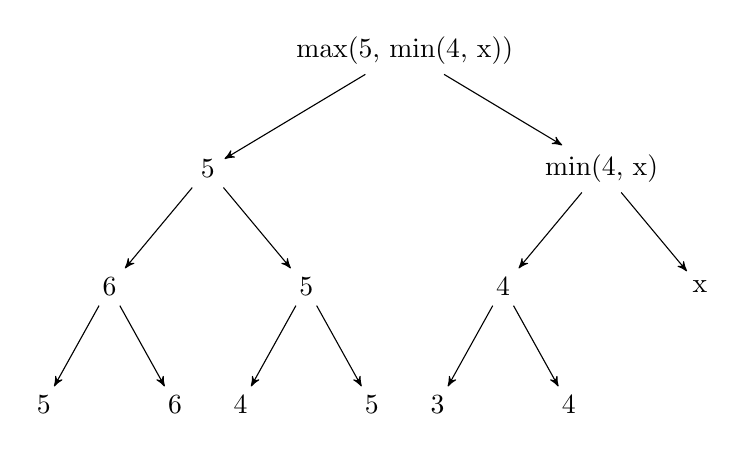
\begin{tikzpicture}[->,>=stealth',level/.style={sibling distance = 5cm/#1,
  level distance = 1.5cm}]
\node {max(5, min(4, x))}
    child{ node {5}
    	child{ node {6}
            child{ node {5}}
            child{ node {6}}
        }
		child{ node {5}
            child{ node {4}}
            child{ node {5}}
        }
    }
    child{ node {min(4, x)}
        child{ node {4}
            child{ node {3}}
            child{ node {4}}
        }
        child{ node {x}}
    }
;
\end{tikzpicture}
\end{center}

Algorytm Alfa-Beta wprowadza pomocniczą funkcję \(alfabeta\):

\[
  \begin{cases}
    alfabeta(v, alfa, beta) \leq alfa    & \quad \text{if } minmax(v) \leq alfa\\
    alfabeta(v, alfa, beta) = minimax(v) & \quad \text{if } alfa < minmax(v) < beta \\
    alfabeta(v, alfa, beta) \geq beta    & \quad \text{if } minmax(v) \geq beta \\
  \end{cases}
\]

Przedział \((alfa, beta)\) nazywany jest oknem przeszukiwania - wartość wewnątrz niego to dokładnie obliczona wartosć \(minimax\).
Dla korzenia za okno przeszukiwania przyjmuje się przedział \((-\infty, \infty)\), a więc oblicza się dokładną wartość \(minimax\).
Znaczenie okna przeszukiwania można wyrazić następującą intuicją: jeżeli wartość obliczana dla danego wierzchołka jest większa niż \(beta\), to końcowy wynik obliczeń nie zmieni się, jeżeli za wartość bieżącego wierzchołka przyjmiemy \(beta\) lub dowolną większą liczbę; gracz \(min\) nie dopuści do rozpatrywanego stanu, ponieważ ma lepszą alternatywę (analogicznie gdy wartość jest mniejsza niż \(alfa\) dla gracza \(max\)).
Sam algorytm wygląda następująco:

\begin{algorithm}
\caption{alfabeta}\label{alfabeta}
\begin{algorithmic}[1]
\Function{alfabeta}{$v, alfa, beta$}
\If {$\texttt{\(v\) jest liściem}$}
	\State \Return $funkcjaOceniajaca(v)$
\EndIf
    \If {\texttt{ruch wykonuje gracz \(max\)}}
    \ForAll {\texttt{\(w\) jest synem \(v\)}}
        \State $alfa \gets max(alfa, alfabeta(w, alfa, beta))$
        \If {$ alfa \geq beta$}
            \State \textbf{break}
        \EndIf
    \EndFor
	\State \Return $alfa$
\Else
    \ForAll {\texttt{\(w\) jest synem \(v\)}}
        \State $beta \gets min(beta, alfabeta(w, alfa, beta))$
        \If {$ alfa \geq beta$}
            \State \textbf{break}
        \EndIf
    \EndFor
	\State \Return $beta$
\EndIf
\EndFunction
\end{algorithmic}
\end{algorithm}

\subsection{Tablica transpozycji}

Ponieważ algorytmy Minimax i Alfa-Beta traktują graf gry jako drzewo, ten sam wierzchołek może być odwiedzony kilkukronie, o ile prowadzą do niego różne ścieżki.
Ta obserwacja jest podstawą techniki tablicy transpozycji, która pozwala na wykorzystanie wyników wcześniejszych obliczeń w trakcie działania algorytmu i przyspieszenie, dzięki któremu można zwiększyć głębokość przeszukiwania.

Zastosowanie tablicy transpozycji wymaga użycia funkcji haszującej \(h\), która umożliwi przypisanie każdemu stanowi gry liczbę całkowitą, ograniczoną z góry przez ustaloną wartość.
Należy też ustalić wielkość tablicy \(R\), która będzie musiała zmieścić się w pamięci dostępnej botowi.
Wtedy, po obliczeniu wartości wierzchołka \(w\), pod indeksem \(h(w)\ \textrm{mod}\ R\) tablicy haszującej umieszcza się wpis zawierający \(h(w)\), odległość wierzhołka \(w\) od korzenia w przeszukiwanym drzewie (wysokość) oraz specyficzne dla algorytmu wartości przydatne przy ponownym odwiedzeniu wierzchołka \(w\).
Zapisana wartość \(h(w)\), podczas odwiedzania wierzchołka \(v\) takiego, że \(h(w) \equiv h(v) (\textrm{mod}\ R)\), pozwala rozpoznać kolizję.
Zapisana wysokość wierzchołka \(w\) określa jakość wpisu.
Wysokość równa głębokości przeszukiwania oznacza, że wierzchołek był odwiedzony jako liść i zapisana wartość jest wprost wartością funkcji oceniającej dla tego wierzchołka.
Taką wartość uznajemy za gorszą od obliczonej dla wysokości o jeden mniejszej, kiedy rozpatrzone zostały wszystkie możliwe kolejne ruchy.
A zatem odnaleziony w tablicy transpozycji wpis może zostać użyty tylko wtedy, gdy zgadzają się wartości funkcji haszującej oraz wysokość zapisana we wpisie jest nie większa niż bieżąca.

W przypadku algorymu Minimimax dodatkowym polem wpisu jest to po prostu obliczona wartość wierzchołka, która może zostać zwrócona po spełnieniu wcześniej wymienionych warunków.

W przypadku algorytmu Alfa-Beta, wpis zawiera ograniczenie dolne i górne na wartość \(minimaks\) wierzchołka (równe sobie, jeżeli znana jest dokładna wartość).
Taki wpis nie zawsze pozwala natychmiast zwrócić wynik, ale może zawęzić okno przeszukiwania i skrócić czas działania algorytmu.

\subsection{Dalsze ulepszenia}

Istnieją dalsze ulepszenia algorytmu Alfa-Beta (NegaScout, MTD-f), które opierają się na zawężaniu okna przeszukiwania.
Ten zabieg skraca czas działania, ale nie musi zwrócić przydatnego wyniku.
Na przykład, zamiast obliczać wartość \(alfabeta(w, alfa, beta)\) oblicza się \(alfabeta(w, alfa, beta')\), gdzie \(alfa < beta' < beta\).
Otrzymana wartość jest poprawnym wynikiem \(alfabeta(w, alfa, beta)\), o ile jest mniejsza od \(beta'\).
Choć obliczanie nieużytecznych wyników spowalnia algorytm, powinno zdarzać się rzadko.
Ostatecznie, skuteczność tych technik sprawdza się eksperymentalnie.

\section{Metody Monte Carlo}

Metoda Monte Carlo nie opiera się w żaden sposób na Minimax i w ogóle nie wymaga użycia funkcji oceniającej wartość wierzchołka.
Do jej zastosowania wystarczy znajomość zasad gry, to znaczy możliwych ruchów dla każdego stanu oraz stanów końcowych wraz z wynikiem rozgrywki.
Ruchy oceniane są na podstawie wyników losowych symulacji; w najprostszym algorytmie, od synów danego wierzchołka moglibyśmy rozpocząć równą ilość losowych rozgrywek i wybrać tego, który najczęściej doprowadził do zwycięstwa.

\subsection{Monte Carlo Tree Search}

W praktyce prosta metoda Monte Carlo nie sprawdza się i należy w trakcie przeprowadzania symulacji niektóre wierzchołki początkowe porzucać jako mało obiecujące, a inne rozwijać, tzn. w ich miejsce wstawić wszystkich synów jako samodzielne wierzchołki początkowe symulacji.
Tak działa Monte Carlo Tree Search (MCTS).

Algorytm ten utrzymuje drzewo, zakorzenione w wierzchołku dla którego wybiera ruch i początkowo posiadające ponad to wyłącznie liść dla każdego możliwego kolejnego stanu gry.
Każdy wierzchołek tego drzewa utrzymuje statystyki symulacji: liczbę symulacji i liczbę symulacji zakończonych zwycięstwem, które rozpoczęły się w poddrzewie danego wierzchołka.
Tak długo jak pozwalają na to limity czasu i pamięci, algorytm przechodzi od korzenia do pewnego liścia wybierając zawsze najbardziej obiecującego syna w zależności od wcześniej zebranych statystyk. Na podstawie statystyk liścia podejmuje decyzję o rozwinięciu go (dodaniu możliwych kolejnych stanów gry do drzewa ze statystykami) i jeśli to zrobi, wybiera jednego z dodanych synów, aby ostatecznie zawsze wybrać liść.
Dalej rozpoczyna od liścia losową rozgrywkę aż do poznania zwycięzcy, po czym aktualizuje statystyki wierzchołków na ścieżce od korzenia do liścia, z którego rozpoczęła się symulacja.
Najlepszy ruch z korzenia wyznacza jego syn, w którego statystykach stosunek zwycięstw do przeprowadzonych symulacji jest najkorzystniejszy.

W opisie algorytmu widać pewne luki: sposób wybierania najbardziej obiecującego syna i kryteria decyzji o rozwinięciu liścia.

Przy wybieraniu nabardziej obiecującego syna używa się metody granicy ufności.
Ma ona zapobiec sytuacji, w której po niewielkiej liczbie symulacji (nawet tylko jednej) liść jest porzucany, co ma miejsce gdy porównuje się wyłącznie stosunek liczby zwycięstw do liczby symulacji.
W tym celu to tego ilorazu dodawany jest tzw. współczynnik ufności, tym wyższy im mniejszą częścią symulacji rodzica są symulacje danego syna. Jako współczynnik ufności przymuje się \(\sqrt{\frac{\sqrt{n_p}}{n_s}}\) lub \(\sqrt{\frac{\log{n_p}}{n_s}}\), gdzie \(n_s\) to liczba symulacji w poddrzewie syna, a \(n_p\) to liczba symulacji w poddrzewie rodzica.

Decyzję o rozwinięciu liścia podejmuje się na podstawie liczby symulacji, jakie zostały z niego rozpoczęte. Jeżeli przekroczy ustalony próg, zwykle zbliżony do liczby ruchów możliwych w jednym stanie gry, liść zostaje rozwinięty.

Oba parametry, tzn. wariant granicy ufności i próg rozwinięcia liścia, ustala się eksperymentalnie.

\chapter{Środowisko bota: tworzona aplikacja}

\section{Doprecyzowanie zasad}

Dla pewnych stanów gry oryginalne zasady nie odpowiadają jednoznacznie na pytanie o legalne ruchy albo dają odpowiedź nieoczekiwaną, wyglądającą na efekt niedopatrzenia. Możliwe, że autorzy i wydawcy gry świadomie woleli pozostawić mało prawdopodobne sytuacje do rozsądzenia graczom niż wydłużać instrukcję analizami kolejnych przypadków, jednak w przypadku tej pracy takie podejście jest niedopuszczalne. Automatyczne testowanie algorytmów sztucznej inteligencji zwiększa prawdopodobieństwo natrafienia na problematyczne stany gry, co może zaburzyć wynik pracy.

\subsection*{Brak legalnych ruchów}

Niech pionki czarny i zielony sąsiadują z pionkiem czerwonym. Dalej, niech pionek czarny będzie odgrodzony od wszystkich sąsiednich pól oprócz tego, na którym stoi czerwony i niech czerwony będzie odgrodzony od tych pól, na których nie stoją czarny ani zielony. Teraz, jeżeli właściciel pionka czarnego nie ma już ogrodzeń, nie może wykonać ruchu.

\begin{figure}[ht!]
\centering
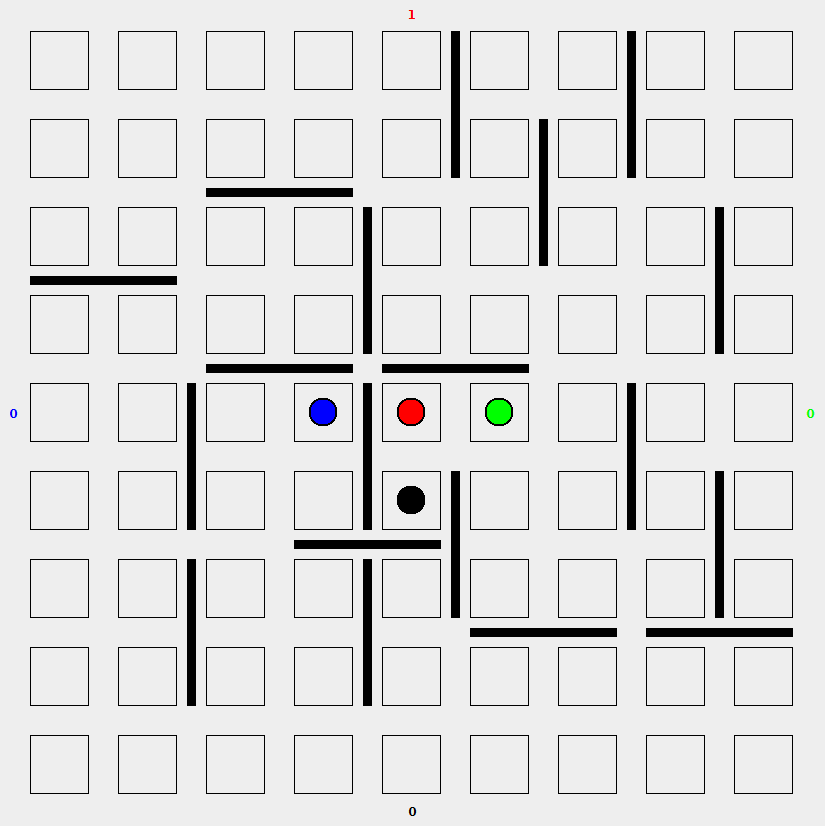
\includegraphics[width=120mm]{img/no-move.png}
\caption{Brak legalnych ruchów \label{overflow}}
\end{figure}

\subsection*{Rozwiązanie problemu braku legalnych ruchów}

TODO

\chapter{Rozwijanie botów}

\chapter{Podsumowanie}

\begin{thebibliography}{99}
\addcontentsline{toc}{chapter}{Bibliografia}
\end{thebibliography}

\end{document}


%%% Local Variables:
%%% mode: latex
%%% TeX-master: t
%%% coding: utf-8
%%% End:
